\chapter{Les factures}
Les factures sont tout comme les devis sont une des fonctionnalités les plus importantes de l'application. De propriétés semblables, il est aussi possible de créer plusieurs factures pour un projet.
\section{Liste des factures\index{Facture!Liste}}
Pour afficher les factures d'un projet il faut comme pour les devis, à partir du panneau contenant la liste des projets d'un client, faire un double clic sur le projet en question. La liste affichée, qui est la même que la liste \ref{fig:creerDevis} contient les factures et les devis du projet sélectionné auparavant.

\section{Ajouter une facture\index{Facture!Ajouter}}
Pour ajouter une facture, il est nécessaire de sélectionner un client dans le panneau central (si l'on est dans la liste des projets ou des factures, la nouvelle facture sera automatiquement ajoutée à ce client). Une fois le client sélectionné on crée une nouvelle facture en cliquant sur le bouton << Nouvelle facture >> de la barre d'outils ou via le menu << Client $\rightarrow$ Nouvelle facture >>. 
\begin{figure}[H]
	\centering
	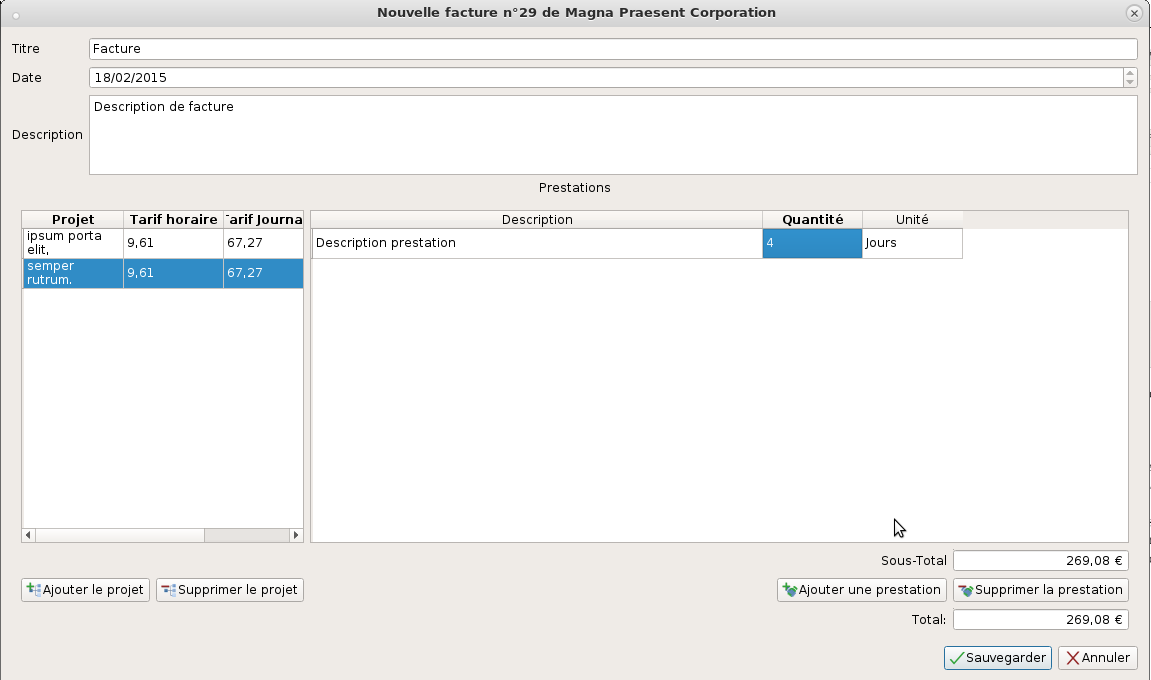
\includegraphics[width=17cm]{screens/creerFacture.png}
	\caption{Créer une nouvelle facture pour un projet client}
	\label{fig:creerFacture}
\end{figure}
Une facture possède :
\begin{enumerate}
	\item un titre à afficher
	\item une date (celle du jour de création du projet)
	\item une description et deux tableaux exactement comme lors de la création ou l'édition d'un devis.
\end{enumerate}	
 Le fonctionnement est le même que pour un devis (cf. \ref*{ch:ajoutDevis}, p \pageref{ch:Prestations}).

Il est également possible de créer une  nouvelle facture à partir d'un existant via le bouton << copier la facture >>. Après ouverture de la fenêtre contenant les informations du modèle, il est possible de changer la nouvelle facture en devis. 
\section{Éditer une facture\index{Facture!Éditer}}
Pour éditer une facture, il faut comme pour un devis, cliquer dessus sur le tableau affichant les devis et les factures d'un projet. Une fois le devis sélectionné, on affiche la fenêtre d'édition de devis en cliquant sur le bouton << Editer la facture >> en dessous du tableau.
La fenêtre qui s'affiche est en tout point semblable à la fenêtre d'ajout d'une facture \ref{fig:creerFacture} hormis le fait que tous les champs sont déjà pré-remplis.
\section{Les Prestations\index{Facture!Prestation}}
Les prestations ont exactement le même comportement que lorsqu'on fait une création ou une édition d'un devis (cf. \ref{ch:Prestations}, p \pageref{ch:Prestations}).